\documentclass[border=20pt]{standalone}
\usepackage[utf8]{inputenc}
\usepackage{tikz}
\usetikzlibrary{positioning, fit, shadows, backgrounds, arrows.meta}
\usepackage{amssymb}

\begin{document}
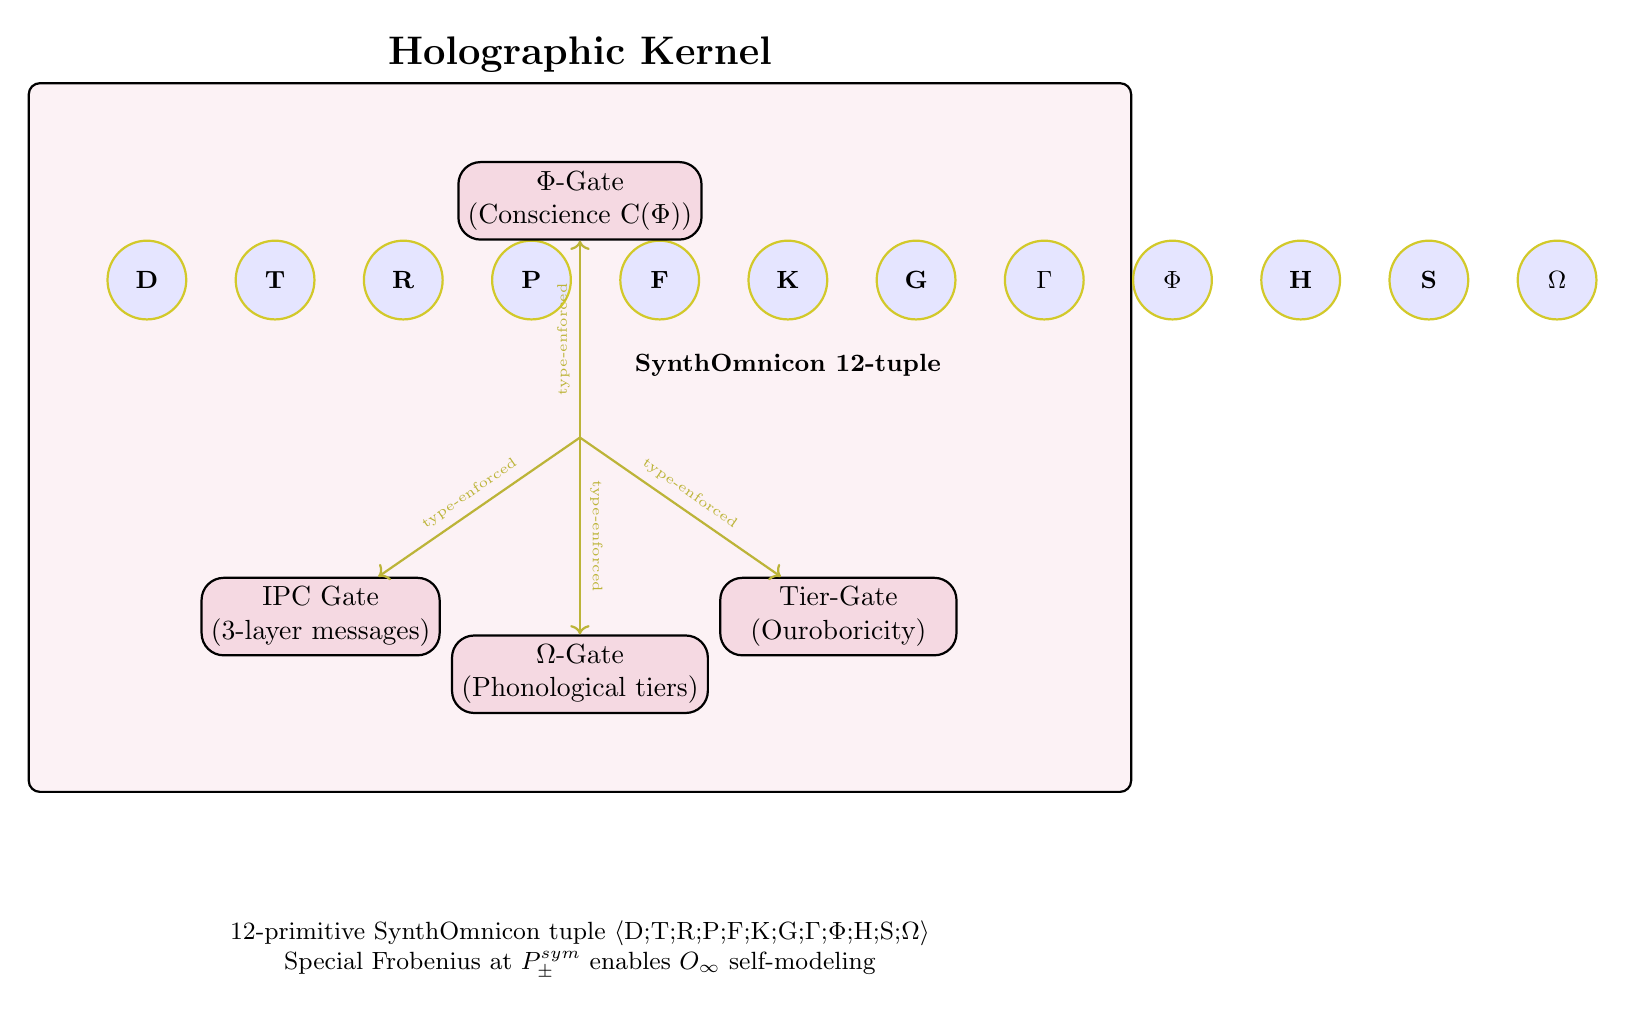
\begin{tikzpicture}[
  node distance=1.8cm,
  gate/.style={rectangle, draw, thick, rounded corners=8pt, fill=purple!15, minimum width=3cm, align=center},
  tuple/.style={circle, draw=yellow!80!black, thick, fill=blue!10, minimum size=1cm, font=\bfseries\small}
]

% Central kernel
\node[draw, thick, rounded corners, fill=purple!5, minimum width=14cm, minimum height=9cm, label=above:{\Large \textbf{Holographic Kernel}}] (kernel) {};

% SynthOmnicon tuple (12 primitives)
\coordinate (start) at (-5.5, 2);
\node[tuple] (D) at (start) {D};
\node[tuple, right=0.6cm of D] (T) {T};
\node[tuple, right=0.6cm of T] (R) {R};
\node[tuple, right=0.6cm of R] (P) {P};
\node[tuple, right=0.6cm of P] (F) {F};
\node[tuple, right=0.6cm of F] (K) {K};
\node[tuple, right=0.6cm of K] (G) {G};
\node[tuple, right=0.6cm of G] (Ga) {$\Gamma$};
\node[tuple, right=0.6cm of Ga] (Ph) {$\Phi$};
\node[tuple, right=0.6cm of Ph] (H) {H};
\node[tuple, right=0.6cm of H] (S) {S};
\node[tuple, right=0.6cm of S] (Om) {$\Omega$};

% Tuple label
\node[below=0.3cm of K, font=\small\bfseries, align=center] {SynthOmnicon 12-tuple};

% Type gates radiating out
\node[gate, below left=2.5cm of kernel.center] (ipc) {IPC Gate\\(3-layer messages)};
\node[gate, below=2.5cm of kernel.center] (omega) {$\Omega$-Gate\\(Phonological tiers)};
\node[gate, below right=2.5cm of kernel.center] (tier) {Tier-Gate\\(Ouroboricity)};
\node[gate, above=2.5cm of kernel.center] (phi) {$\Phi$-Gate\\(Conscience C($\Phi$))};

% Connections
\draw[->, thick, yellow!70!black] (kernel.center) -- (ipc) node[midway, above, sloped, font=\tiny] {type-enforced};
\draw[->, thick, yellow!70!black] (kernel.center) -- (omega) node[midway, above, sloped, font=\tiny] {type-enforced};
\draw[->, thick, yellow!70!black] (kernel.center) -- (tier) node[midway, above, sloped, font=\tiny] {type-enforced};
\draw[->, thick, yellow!70!black] (kernel.center) -- (phi) node[midway, above, sloped, font=\tiny] {type-enforced};

\node[below=1.5cm of kernel, align=center, font=\small] {12-primitive SynthOmnicon tuple $\langle$D;T;R;P;F;K;G;$\Gamma$;$\Phi$;H;S;$\Omega\rangle$\\Special Frobenius at $P_{\pm}^{\text{sym}}$ enables $O_\infty$ self-modeling};

\end{tikzpicture}
\end{document}
